\chapter{Design Description}
\label{design-description}

\begin{remark}\color{blue}
The description section defines what the design is. If you find yourself adding rationale, or discussing design alternatives, you are writing text that should be moved into the Development section. A few teams find that this section fits more naturally if it comes before the Design Development section.

In the Fall quarter, the design will be in an early stage and this section is largely a proposal for what the design should be (you can call it that, explicitly). Even so, on the basis of preliminary need-finding, benchmarking and critical function evaluation, you have some idea of what is appropriate. Take a point of view and assert it. A CAD model or systems diagram of a concept may be appropriate.
\normalcolor \end{remark}

\section{Vision}
\label{vision}

\begin{remark}\color{blue}
Use this section to describe your vision or proposal for what you think the design might be. Ideally you should have a sketch, a diagram or other images to help define it.
\normalcolor\end{remark}

The remaining text in this section contains of excerpts from the Autodesk 2007-08 Fall document \cite{Autodesk2008Fall}.

\section{Tactile Messaging CFP}

The tactile messaging system was comprised of small Jameco vibrating motors (1.3VDC 8,500 RPM) mounted to ball point pens and wrist patches. A simple switchable voltage supply circuit was created to give each vibrating motor a high (1.2V) and low (0.6V) vibrating speed (\ref{fig:tactile_circuit}). Each voltage level was buffered with LM324 opamps, and the circuits were implemented on protoboards. The high and low speeds were selected by switches. 

\begin{figure}[bhtp] 
	\begin{center}
		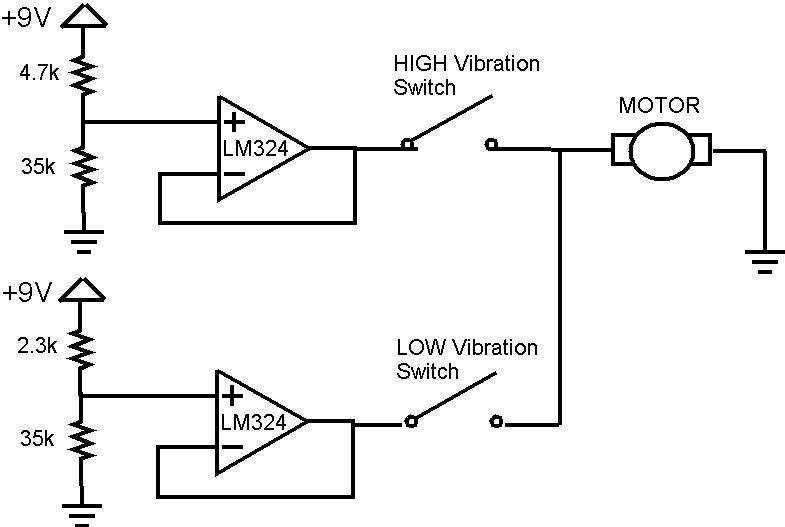
\includegraphics[width= \figwidth]{Figures/Ch5/tactile_circuit.jpg}
	\end{center}
	\caption[voltage divider]{A simple voltage dividing circuit provided 1.2V (HIGH) and 0.6V (LOW) buffered output voltages for the vibrating motor. Switches triggered the high and low voltages. }
	\label{fig:tactile_circuit}  
\end{figure}

\begin{center}
\color{blue}
(Text omitted for brevity)
\normalcolor
\end{center}

Four independent circuits were created to provide messaging to two motors on each side. 90' 16-gauge wire was passed between two stations in the meeting setup shown in \ref{fig:tactile_seating}. Power supplies provided the 9V signal on each side.

\begin{figure}[bhtp] 
	\begin{center}
		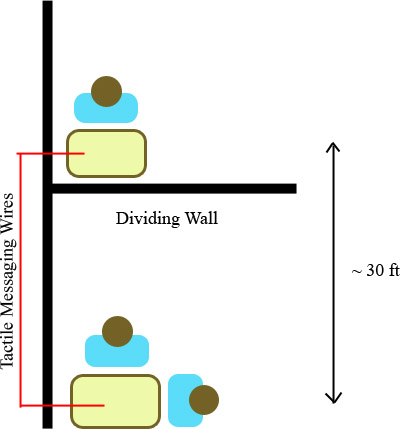
\includegraphics[width=3in]{Figures/Ch5/tactile_seating.jpg}
	\end{center}
	\caption[test meeting layout]{Layout of seating during test meeting. Two participants met on one side, with the remote user separated by a wall 50 ft away. }
	\label{fig:tactile_seating}  
\end{figure}

In addition to the tactile hardware, Skype was used for video and audio communication. Video was supplied by standard webcams. We mounted the webcams on risers to show video of a sheet of white paper used as the shared drawing space. We chose to focus the video on ideas rather than facial expressions. 


\clearpage
\section{Moderator CFP}

\subsection{Layout}

The participation moderator was created by using pre-made desktop software applications called widgets. The desktop was set to a white image, with personal spaces for each participant mapped off by a black boundary and labelled with the participant name. In each personal space, a unique Yahoo! Widgets timer was placed. Unique timer's were used to foster a sense of identity- when glancing at the moderator, the team members could instantly recognize their widget rather than look for their name. 

\begin{figure}[htbp]
	\centering
		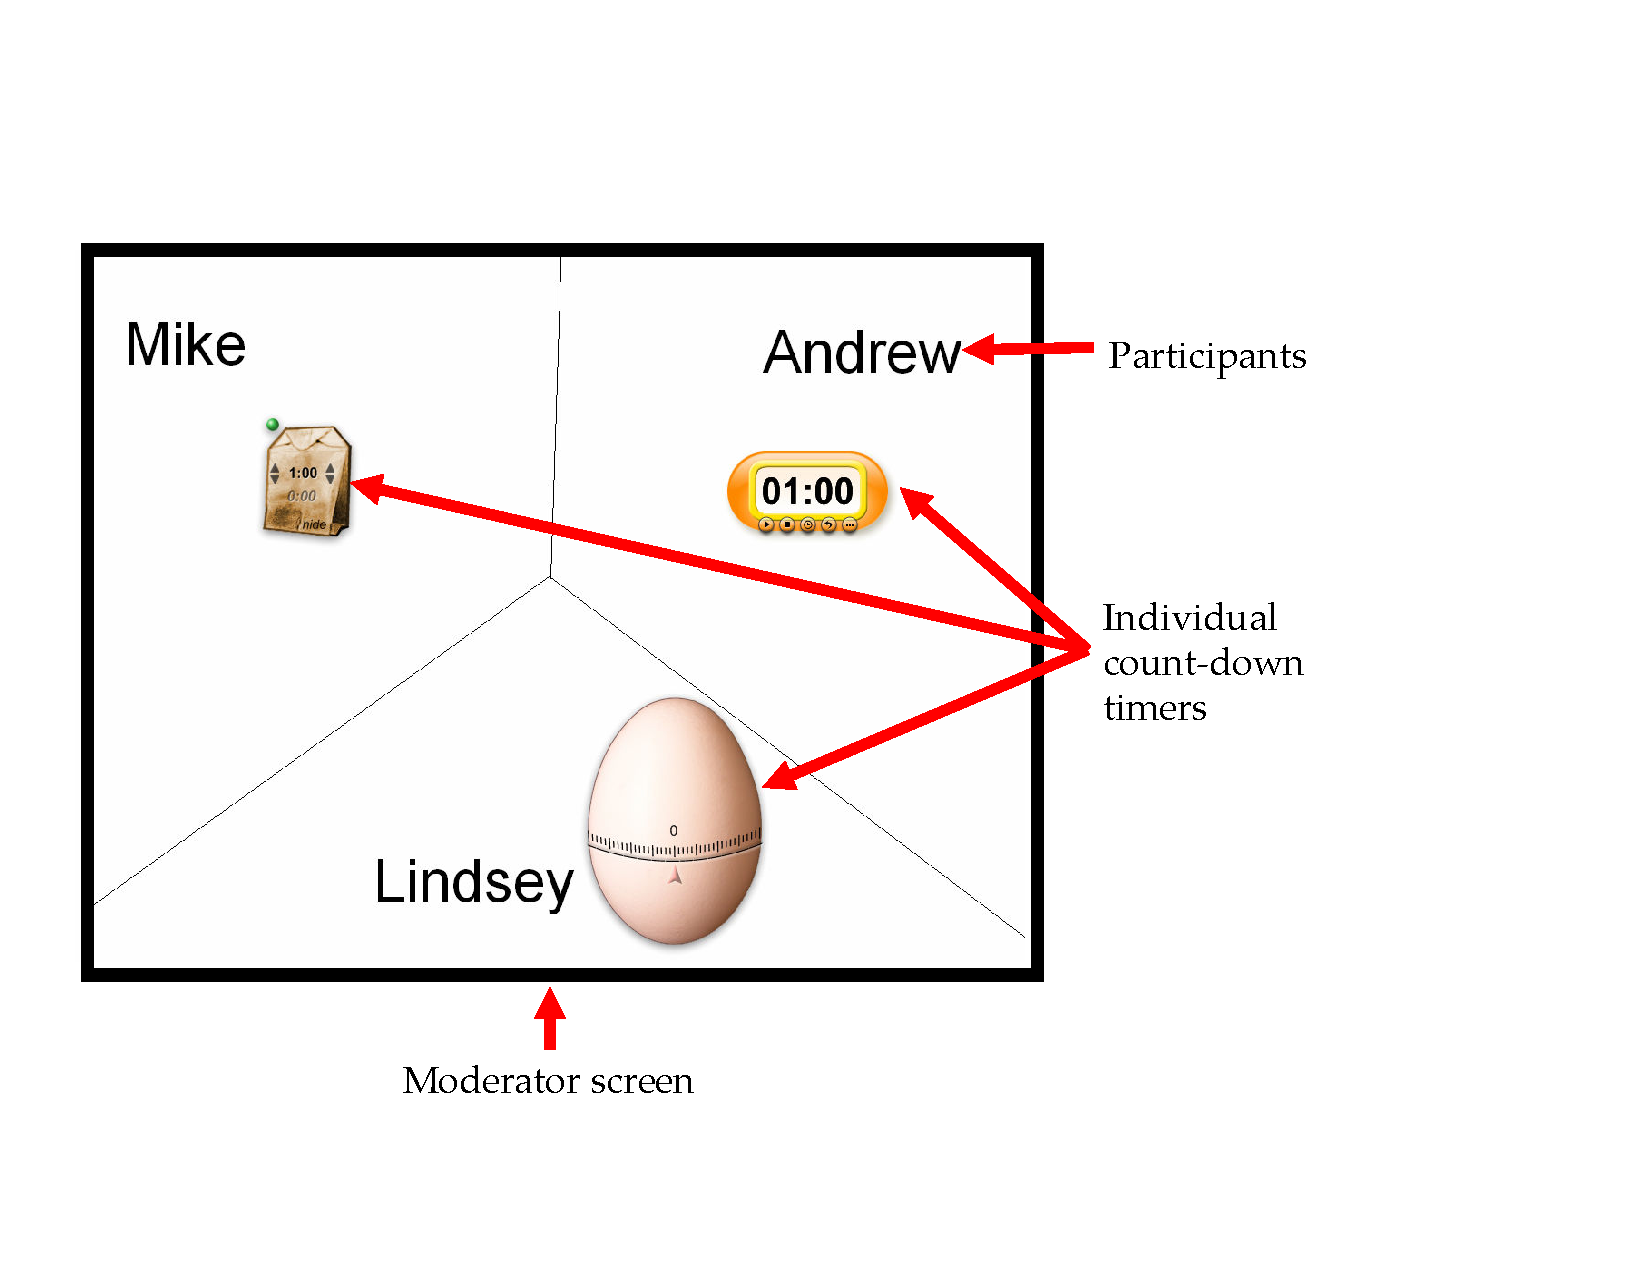
\includegraphics[width=1.00\textwidth]{Figures/Ch5/moderator.pdf}
	\caption{View of moderator display}
	\label{fig:moderator}
\end{figure}

\begin{center}
\color{blue}
(Text omitted for brevity)
\normalcolor
\end{center}


Each was simply a countdown timer with a default starting time, $t_{s}$. As they begin counting down, the amount of time remaining is visible. By clicking twice on any widget, it would reset and begin counting down again from $t_{s}$. The timers were manually reset by one of the teammates during the meeting whenever someone had an interaction. When any timer runs out, it would sound an alarm, designating that the meeting come to a halt until the non-active team member contributes to the conversation. The hypothesis was that, because the timers were visible to the entire team, each member would consciously make an effort to speak before their timer ran out and that no timer would actually buzz, although the rotation of speakers would greatly increase.

The moderator screen was displayed on a 32" LCD display that was positioned 6' from the center of a table where the group met. The layout is detailed in Figure \ref{fig:moderator_setup}. No video or audio conferencing was used -- all team members were local. The objective of the moderator is to support dialogue in meetings, regardless of whether the members are distributed or not. Audio was recorded of each meeting using Cubase software and an IBM laptop's internal microphone, which was placed in the center of the table so each participant could be heard. 

\begin{figure}[h]
	\centering
		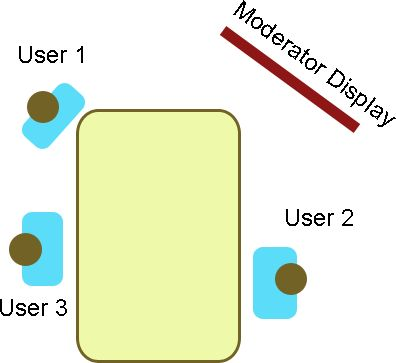
\includegraphics[width=.75\textwidth]{Figures/Ch5/moderator_setup.jpg}
	\caption{Layout of design meeting with moderator prototype}
	\label{fig:moderator_setup}
\end{figure}

\subsection{Procedure}

Three meetings were run to test the moderator. The subject of each was the same - our team brainstormed potential final products knowing the key lessons learned after our benchmarking. Three meetings were run in succession, each lasting 30 minutes. The intention of this was to eliminate any personal changes between meetings. For example, if Mike has a really bad day before coming in for a second meeting, he may be much less talkative than in the previous meeting, but not as a result of the moderator. The first meeting served as the control, and no moderator was used. The two subsequent meetings used the moderator with $t_{s}$ at 2 minutes and 1 minute.

The audio files were analyzed manually by playing back the audio recordings for each meeting and recording the length of each comment that every person made. Fifteen minutes of audio during the middle of each meeting was processed. The data are available in Appendix \ref{sec:Appendix1}. 


